\chapter{Conclusiones}\label{cap:conclusiones}
Una vez finalizado el trabajo, con el self-hosted runner contenerizado con Docker, y teniendo el microcontrolador conectado por cable microUSB a la computadora que actúa como servidor para correr el runner, se está en condiciones de modificar el código del programa desde cualquier lugar con acceso a internet. En esta aplicación sencilla se espera únicamente un cambio en la frecuencia de parpadeo del LED.

Una vez que se pushean al repositorio cambios en las carpetas /src, /include y /tests de la rama principal, se desencadenan las tareas del Workflow para compilar, testear y cargar el nuevo programa en la placa.

\textbf{Consumo de Recursos}

Se midió el consumo de recursos de esta aplicación sencilla para la placa, gracias a la funcionalidad de PlatformIO Statistics, obteniendo las métricas de uso de memoria RAM, uso de almacenamiento Flash, y defectos encontrados, las cuales se muestran en la figura \ref{fig:metrics}.

\begin{figure}[H]
    \centering
    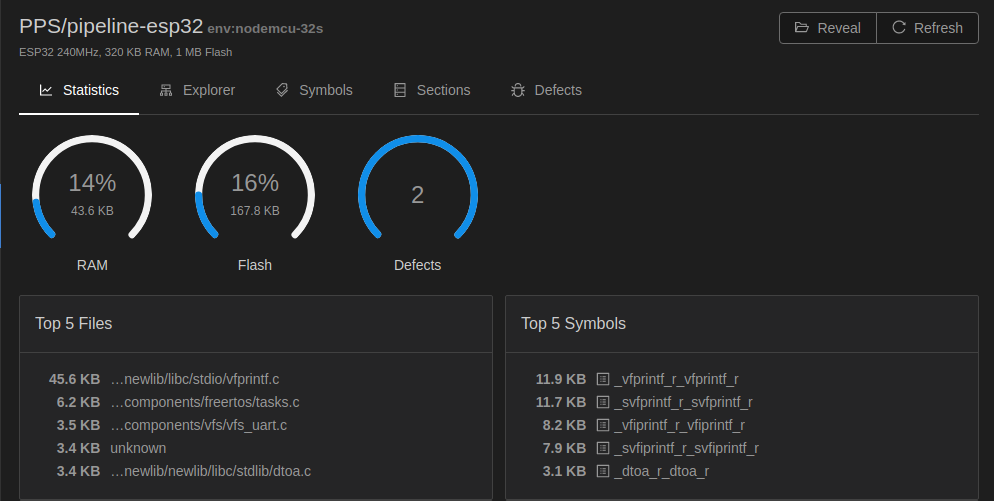
\includegraphics[width=1\textwidth]{fig/platformio-esp32-metrics.png}
    \caption{Métricas del ESP32 corriendo la aplicación}
    \label{fig:metrics}
\end{figure}

\textbf{Tiempos}

La ejecución inicial del runner demora aproximadamente 2 minutos hasta que está listo para ejecutar jobs.
Cuando se pushea un cambio por primera vez, se demora bastante para instalar las dependencias en el contenedor, aproximadamente unos 8 minutos. Para posteriores pusheos de cambios, se corren los jobs más rápidamente porque el contenedor ya tiene sus dependencias instaladas, en este caso demora aproximadamente 2 minutos en cargar el nuevo código en la placa, considerando que pasaron exitosamente los tests. Se resume esta información en la tabla

\begin{table}[H]
\begin{center}
\begin{tabular}{lll}
\hline
\multicolumn{1}{|l|}{\textbf{Caso}} & \multicolumn{1}{l|}{\textbf{Tiempo aproximado}} \\ \hline
\multicolumn{1}{|l|}{Ejecución Inicial del Runner con Docker} & \multicolumn{1}{l|}{2 minutos} \\ \hline
\multicolumn{1}{|l|}{Workflow Jobs al recibir el primer push} & \multicolumn{1}{l|}{8 Minutos} \\ \hline
\multicolumn{1}{|l|}{Workflow Jobs al recibir los siguientes pushes} & \multicolumn{1}{l|}{2 Minutos} \\ \hline
\end{tabular}
\caption{Tiempos del GitHub Runner en ejecutar las tareas del Workflow}
\label{tab:multiplicadores-minutos}
\end{center}
\end{table}

Los tiempos dependen de la computadora con la que se corre el self-hosted runner, en este caso se trata de una notebook de gama media del año 2020, modelo Lenovo Legión 5i, cuya ficha técnica se puede encontrar en el siguiente \href{https://www.lenovo.com/ar/es/laptops/laptops-legion/legion-5-series/Legion-5i-15/p/88GMY501434}{enlace}.


